% Copyright 2004 by Till Tantau <tantau@users.sourceforge.net>.
%
% In principle, this file can be redistributed and/or modified under
% the terms of the GNU Public License, version 2.
%
% However, this file is supposed to be a template to be modified
% for your own needs. For this reason, if you use this file as a
% template and not specifically distribute it as part of a another
% package/program, I grant the extra permission to freely copy and
% modify this file as you see fit and even to delete this copyright
% notice.

\documentclass{beamer}

% There are many different themes available for Beamer. A comprehensive
% list with examples is given here:
% http://deic.uab.es/~iblanes/beamer_gallery/index_by_theme.html
% You can uncomment the themes below if you would like to use a different
% one:
%\usetheme{AnnArbor}
%\usetheme{Antibes}
%\usetheme{Bergen}
%\usetheme{Berkeley}
%\usetheme{Berlin}
%\usetheme{Boadilla}
%\usetheme{boxes}
%\usetheme{CambridgeUS}%%%%%%%%%%%%%%%%%%%%%%%%%%%%%%
%\usetheme{Copenhagen}
%\usetheme{Darmstadt}
%\usetheme{default}
%\usetheme{Frankfurt}
%\usetheme{Goettingen}
%\usetheme{Hannover}
%\usetheme{Ilmenau}
%\usetheme{JuanLesPins}
%\usetheme{Luebeck}
\usetheme{Madrid}%%%%%%%%%%%%%%%%%
%\usetheme{Malmoe}
%\usetheme{Marburg}
%\usetheme{Montpellier}
%\usetheme{PaloAlto}
%\usetheme{Pittsburgh}
%\usetheme{Rochester}
%\usetheme{Singapore}
%\usetheme{Szeged}
%\usetheme{Warsaw}
%%
%%
%
\setbeamertemplate{theorems}[numbered]
\setbeamertemplate{caption}[numbered]

%use package
\usepackage{multirow}
\usepackage{hyperref}
\usepackage{amssymb}
\usepackage{graphicx}
%\usepackage{algorithm}
\usepackage{amsmath,amsfonts}
\usepackage{amsthm}
\usepackage{amsmath}
\usepackage{xcolor}
\usepackage{dsfont}
\usepackage{epsfig}
\usepackage{color}
\usepackage{textcomp}
%\usepackage{beamerthemesplit}
%\usepackage{{ntheorem}}
%\usepackage[justification=centering]{caption}
%\usepackage{subfigure}% Support for small, `sub' figures and tables
\usepackage{subcaption}
\usepackage[utf8]{inputenc}
%\usepackage{tikz}
%\usepackage[tightpage]{preview}
%\usepackage{cite}
%\usepackage[scaled]{helvet}
%\usepackage[round]{natbib}
%%%<
%\usepackage{verbatim}
\usepackage[ruled,vlined]{algorithm2e} % package for algorithms.
\usepackage{multimedia} % package for multimedia, uo
\SetAlFnt{\tiny}
%%%%
%
%\logo{
\includegraphics[height=1cm]{logo.png}\vspace{220pt}}
%\logo{
\includegraphics[height=1cm]{logo.png}}

\title[Robot Walking by RL]{Bipedal Robot Walking by Reinforcement Learning in Partially Observed Environment}

% A subtitle is optional and this may be deleted
%\subtitle{Optional Subtitle}

\author[U. Özalp]{Uğurcan Özalp*\inst{1}}
% - Give the names in the same order as the appear in the paper.
% - Use the \inst{?} command only if the authors have different
%   affiliation.

\institute[METU] % (optional, but mostly needed)
{
	\inst{1}
	Scientific Computing
%  \inst{1}%
%	Financial Mathematics
%	\inst{2}%
%		Actuarial Sciences
%	\inst{3}
%	Scientific Computing\\
	
	Institute of Applied Mathematics\\
  Middle East Technical University\\
	
 	}
% - Use the \inst command only if there are several affiliations.
% - Keep it simple, no one is interested in your street address.

\date[Thesis Presentation]{Thesis Presentation\\
\today}
% - Either use conference name or its abbreviation.
% - Not really informative to the audience, more for people (including
%   yourself) who are reading the slides online

\subject{DEEP REINFORCEMENT LEARNING}
% This is only inserted into the PDF information catalog. Can be left
% out.

% If you have a file called "university-logo-filename.xxx", where xxx
% is a graphic format that can be processed by latex or pdflatex,
% resp., then you can add a logo as follows:

 \pgfdeclareimage[height=1cm]{university-logo}{logo.jpg}
 \logo{\pgfuseimage{university-logo}}

% Delete this, if you do not want the table of contents to pop up at
% the beginning of each subsection:
%\AtBeginSubsection[]
%{
%  \begin{frame}<beamer>{Outline}
%    \tableofcontents[currentsection,currentsubsection]
%  \end{frame}
%}

% Let's get started
\begin{document}

\begin{frame}
  \titlepage
\end{frame}

\begin{frame}{Outline}
  \tableofcontents
  % You might wish to add the option [pausesections]
\end{frame}

% Section and subsections will appear in the presentation overview
% and table of contents.

\section{Introduction}

\begin{frame}
\frametitle{Introduction}
In this thesis, we investigate;
\begin{itemize}
	\item Performance of varying Neural Network architectures
	\item Deep Reinforcement Learning methods
	\item Environmental settings
\end{itemize}
for bipedal robot walking on \textit{BipedalWalker-Hardcore-v3}~ \cite{noauthor_bipedalwalkerhardcore-v2_2021} environment from open source Gym~\cite{brockman_openai_2016} library of OpenAI.
\end{frame}

%%%%%%%%%%%%%%%%%%%%
%%%%%%%%%%%%%%%%%%%%

\section{Environment}

\begin{frame}
\frametitle{BipedalWalker-Hardcore-v3}
\textit{BipedalWalker-Hardcore-v3} environment is;
\begin{itemize}
	\item Agent has deterministic dynamics, but terrain is randomly generated.
	\item Observation space consists of kinematic observations and lidar rangefinders.
	\item Action space has torque actions from knee and joints.
\end{itemize}
However, walking is a hard control problem due to following reasons.
\begin{itemize}
	\item The dynamics are nonlinear, unstable and multimodal. The terrain where the robot walks also varies. 
	\item Overcoming some obstacles requires a specific maneuver, which is hard to explore sometimes (Sparse Rewards).
	\item The robot observes ahead with lidar measurements and cannot observe behind (Partial observability).
	Also, it lacks of acceleration sensors. 
\end{itemize}
\end{frame}

\begin{frame}
\begin{figure}
\centering
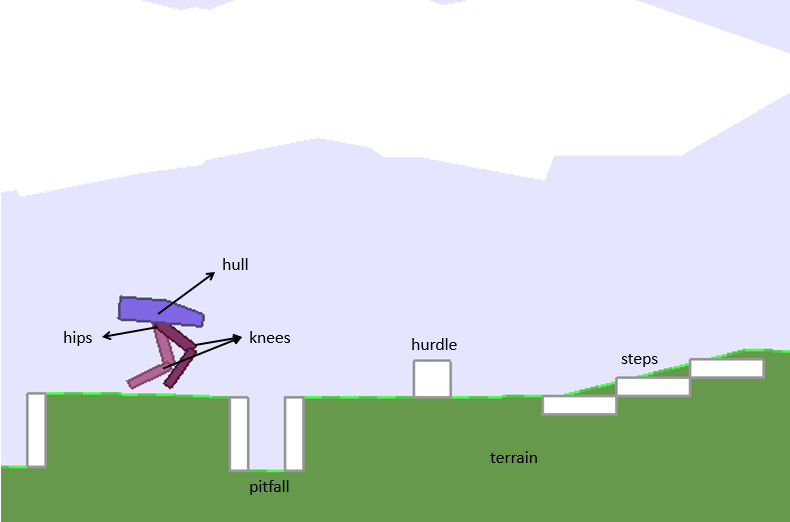
\includegraphics[width=0.95\textwidth]{figures/bipedal/bpedal_annotated.png}
\caption{Bipedal Walker Hardcore Components~\cite{noauthor_bipedalwalkerhardcore-v2_2021}}
\label{fig:bipedal_hardcore_components}
\end{figure}
\end{frame}

%%%%%%%%%%%%%%%%%%%%
%%%%%%%%%%%%%%%%%%%%

\section{Reinforcement Learning}

\begin{frame}
\frametitle{Reinforcement Learning}
The closest kind of learning demonstrated by humans and animals. 
Unline other learning paradigms, a RL agent must;
\begin{itemize}
	\item learn in dynamic environment
	\item gather data itself
	\item make mistakes (exploration)
	\item get reward (exploitation)
	\item understand reason of consequences
	\item keep safe
\end{itemize}
\end{frame}

\begin{frame}
\frametitle{Sequential Decision Making}
\begin{columns}[onlytextwidth]
	\begin{column}{.45\textwidth}
		At time $t$, the agent;
		\begin{itemize}
			\item is in state $s_t \in \mathcal{S}$
			\item gets observation $o_t \in \mathcal{O}$
			\item takes action $a_t \in \mathcal{A}$ depending on policy $\pi$
			\item rewarded by $r_t \in \mathbb{R}$
			\item transitions to state $s_{t+1} \in \mathcal{S}$
			\item gets observation $o_{t+1} \in \mathcal{O}$
		\end{itemize}
	\end{column}
	\begin{column}{.45\textwidth}
		\begin{figure}
			\centering
			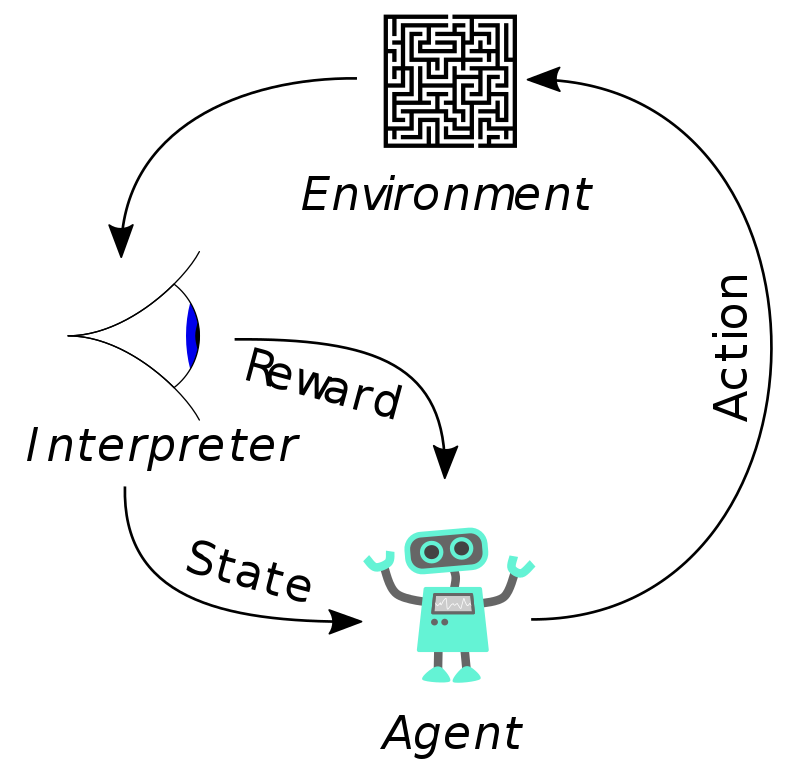
\includegraphics[width=0.95\textwidth]{figures/ml_theory/RL_diagram.png}
			\caption{Reinforcement Learning Diagram}
			\label{fig:rl_diagram}
		\end{figure}
	\end{column}
\end{columns}
\end{frame}

\begin{frame}
\frametitle{Learning}
Learning is obtaining either;
\begin{itemize}
	\item stochastic policy: $\pi: \mathcal{S}\times\mathcal{A} \rightarrow [0,1]$, or
	\item deterministic policy: $\mu: \mathcal{S}\rightarrow\mathcal{A}$
\end{itemize}
by maximizing expected cumulative sum of future rewards, i.e. state-action value function ($Q$), scaled by discount factor $\gamma \in [0,1]$;
\begin{equation}
Q^{\pi}(s,a) = \mathbb{E}\bigg[\sum_{i=t}^{\infty} \gamma^{i-t} r_i|s_t=s, a_t=a, \pi\bigg]. %\quad \forall t = 0,1, ...
\end{equation}
for given any state and actions. \\
For a given model $T$, optimal policy $\pi^*$ and $Q^{\pi^*}$ function should satisfy following Bellman Equation;
\begin{equation}
\label{eqn:bellman_q}
Q^{\pi^*}(s,a) = \mathbb{E}[r|s,a] + \gamma \max_{a'} \Big\{ \sum_{s'} T(s'|s,a) Q^{\pi^*}(s',a') \Big\}
\end{equation}
\end{frame}

%%%%%%%%%%%%%%%%%%%%

\subsection{Deep Q Learning}

\begin{frame}
\frametitle{Q Learning}
Optimizing $Q$ function using Bellman Equation \ref{eqn:bellman_q}.\\
Assume that $Q$ is parametrized function by $\theta$.
Target $Q$ value is estimated by bootstrapping estimate, 
\begin{equation}
\label{eqn:q_target}
Y_t^Q = r_t + \gamma \max_{a'} Q(s_{t+1},a';\theta).
\end{equation}
Minimize difference between the target value and the estimated value, hence the following loss,
\begin{equation}
\label{eqn:q_loss}
\mathcal{L}_t(\theta) = \big( Y_t - Q(s_t,a_t;\theta) \big) ^ 2.
\end{equation}
\end{frame}

\begin{frame}
\frametitle{Deep Q Learning}
In order to stabilize learning, Deep Q Learning~\cite{mnih_human-level_2015, mnih_playing_2013} introduces;
\begin{itemize}
	\item Target Network (parametrized by $\theta^-$) to evaluate target value. Updated at fixed number of steps ($\theta^- \leftarrow \theta$, if $t\mod d = 0$).
	\begin{equation}
	\label{eqn:dqn_ntarget}
	Y_t^{DQN} = r_t + \gamma \max_{a'} Q(s_{t+1},a';\theta^-).
	\end{equation}
	\item Experience Replay $\mathcal{D}$, to store experience tuples $s_t,a_t,r_t,s_{t+1}$ to sample each iteration for loss construction. 
	\begin{equation}
	\label{eqn:dqn_loss}
	\mathcal{L}_i(\theta_i) = \mathbb{E}_{s,a,r,s'\sim U(\mathcal{D})}\Big[\big( Y^{DQN} - Q(s,a;\theta_i) \big) ^ 2 \Big].
	\end{equation}
	\item Epsilon Greedy Exploration, to let agent explore environment. 
	\begin{equation}
	\label{eqn:egreedy_policy}
	\pi(a|s) = 
	\begin{cases}
	1-\epsilon,   & \text{if } a = \arg \max_{a} Q(s, a), \\
	\frac{\epsilon}{|\mathcal{A}|-1},     & \text{otherwise}.
	\end{cases}
	\end{equation}
\end{itemize}
\end{frame}
%%%%%%%%%%%%%%%%%%%%
\subsection{Deep Deterministic Policy Gradient}
\begin{frame}
\frametitle{Deep Deterministic Policy Gradient}
Continuous complement of DQN using a deterministic policy~\cite{lillicrap_continuous_2019}. It is;
\begin{itemize}
	\item Actor critic algorithm (both value and policy parametrized), $\theta^{\mu}$ and $\theta^{Q}$, with target networks $\theta^{\mu^-}$ and $\theta^{Q^-}$. 
	\item Target networks are updated by Polyak averaging ($\tau \in (0,1)$),
	\begin{equation}
	\label{eqn:target_update}
	\theta^- \leftarrow \tau \theta + (1-\tau) \theta^- .
	\end{equation}
	\item For exploration, a random process $\mathcal{X}$ noise added to policy. Typically Ornstein-Uhlenbeck Process (AR(1) process) \cite{uhlenbeck_theory_1930} or Gaussian White Noise is used.
\end{itemize}
\end{frame}

\begin{frame}
\begin{algorithm}[H]
	\SetAlgoLined
	\DontPrintSemicolon % Some LaTeX compilers require you to use \dontprintsemicolon instead
	Initialize: $\mathcal{D}$, $N$, $N_{replay}$, $\theta^{\mu}$, $\theta^Q$, $\mathcal{X}$ \\
	$\theta^{\mu^-} \leftarrow \theta^{\mu}$, $\theta^{Q^-} \leftarrow \theta^{Q}$ \\
	\For{$\text{episode} = 1, M $}{
		Recieve initial state $s_1$; \\
		\For{$t = 1, T$}{
			Select action $a_t = \mu(s_t; \theta^{\mu}) + \epsilon$ where $\epsilon \sim \mathcal{X}$; \\
			Execute action $a_t$ and recieve reward $r_t$ and next state $s_{t+1}$; \\
			Store experience tuple $e_t = (s_t, a_t, r_t, s_{t+1})$ to $\mathcal{D}$ ; \\
			Sample random batch $\mathcal{D}_{r}$ ($|\mathcal{D}_{r}|=N$) from $\mathcal{D}$; \\
			$Y_j = \begin{cases}
			r_j & \text{if } s_{j+1} \text{ terminal } \\
			r_j + \gamma Q(s_{j+1},\mu(s_{j+1}; \theta^{\mu^-}); \theta^{Q^-}) & \text{otherwise }
			\end{cases}$ \qquad $\forall e_j \in \mathcal{D}_{r}$ \\
			Update $\theta^Q$ by minimizing $ \frac{1}{N}\sum_{e_j \in \mathcal{D}_{r}} \big( Y_j - Q(s_j,a_j;\theta^Q) \big) ^ 2$ for a single step; \\
			Update $\theta^{\mu}$ by maximizing $ \frac{1}{N}\sum_{e_j \in \mathcal{D}_{r}} Q(s_j,a_j;\theta^Q)$ for a single step; \\
			Update target networks: \\
			$\theta^{\mu^-} \leftarrow \tau \theta^{\mu} + (1-\tau) \theta^{\mu^-}$ and \\
			$\theta^{Q^-} \leftarrow \tau \theta^{Q} + (1-\tau) \theta^{Q^-}$;
		}
	}
	\caption{Deep Deterministic Policy Gradient}
	\label{alg:ddpg}
\end{algorithm}
\end{frame}

%%%%%%%%%%%%%%%%%%%%

\subsection{Twin Delayed Deterministic Policy Gradient}
\begin{frame}
\frametitle{Twin Delayed Deep Deterministic Policy Gradient}
Improved version of Deep Deterministic Policy Gradient \cite{fujimoto_addressing_2018}.
Upon DDPG, it introduces;
\begin{itemize}
	\item Target Policy Smoothing to regularize network,
	\begin{equation}
	\label{eqn:td3_target_action}
	\widetilde{a}' = \mu(s';\theta^{\mu^-}) + \text{clip}(\epsilon, -c, c), \quad \epsilon \sim \mathcal{N}(0, \sigma^2).
	\end{equation}
	\item Clipped Double Q Learning to prevent Q value overestimation,
	\begin{equation}
	\label{eqn:td3_target}
	Y_t^{TD3} = r_t + \gamma \min_{k\in\{1,2\}} Q(s_{t+1}, ;\widetilde{a}_{j+1};\theta^{Q_k^-}).
	\end{equation}
	\item Delayed Policy Updates to delay policy learning compared to value learning; i.e, learn policy if $t\mod d = 0$
\end{itemize}
\end{frame}

\begin{frame}
\begin{algorithm}[H]
	\SetAlgoLined
	\DontPrintSemicolon % Some LaTeX compilers require you to use \dontprintsemicolon instead
	Initialize: $\mathcal{D}$, $N$, $N_{replay}$, $\theta^{\mu}$, $\theta^Q_1$, $\theta^Q_2$, $\mathcal{X}$, $\sigma$, $c$, $d$ \\
	$\theta^{\mu^-} \leftarrow \theta^{\mu}$, $\theta^{Q^-}_1 \leftarrow \theta^{Q}_1$, $\theta^{Q^-}_2 \leftarrow \theta^{Q}_2$ \\
	\For{$\text{episode} = 1, M $}{
		Recieve initial state $s_1$; \\
		\For{$t = 1, T$}{
			Select action $a_t = \mu(s_t; \theta^{\mu}) + \epsilon$ where $\epsilon \sim \mathcal{X}$
			Execute action $a_t$ and recieve reward $r_t$ and next state $s_{t+1}$; \\
			Store experience tuple $e_t = (s_t, a_t, r_t, s_{t+1})$ to $\mathcal{D}$ ; \\
			Sample random batch $\mathcal{D}_{r}$ ($|\mathcal{D}_{r}|=N$) from $\mathcal{D}$; \\
			Sample target actions for value target,
			$\widetilde{a}_{j+1} = \mu(s_{j+1};\theta^{\mu^-}) + \text{clip}(\epsilon, -c, c), \quad \epsilon \sim \mathcal{N}(0, \sigma^2) \quad \forall e_j \in \mathcal{D}_{r}$; \\
			$Y_{jk} = \begin{cases}
			r_j & \text{if } s_{j+1} \text{ terminal } \\
			r_j + \gamma Q(s_{j+1},\widetilde{a}_{j+1}); \theta^{Q^-}_k) & \text{otherwise } 
			\end{cases}$ \qquad $\forall e_j \in \mathcal{D}_{r}$, $\forall k \in \{1,2\}$ \\
			$Y_j = \min(Y_{j1}, Y_{j2})$; \\
			Update $\theta^Q_1$ $\theta^Q_2$ by seperately minimizing $ \frac{1}{N}\sum_{e_j \in \mathcal{D}_{r}} \big( Y_j - Q(s_j,a_j;\theta^Q_k) \big) ^ 2 \quad \forall k \in \{1,2\}$ for a single step; \\
			\uIf{$t \mod d$}{
				Update $\theta^{\mu}$ by maximizing $ \frac{1}{N}\sum_{e_j \in \mathcal{D}_{r}} Q(s_j,a_j;\theta^Q_1)$ for a single step; \\
				Update target networks: \\
				$\theta^{\mu^-} \leftarrow \tau \theta^{\mu} + (1-\tau) \theta^{\mu^-}$ and \\
				$\theta^{Q^-}_k \leftarrow \tau \theta^{Q}_k + (1-\tau) \theta^{Q^-}_k \quad \forall k \in \{1,2\}$ ;
			}
		}
	}
	\caption{Twin Delayed Deep Deterministic Policy Gradient}
	\label{alg:td3}
\end{algorithm}
\end{frame}

%%%%%%%%%%%%%%%%%%%%

\subsection{Soft Actor-Critic}
\begin{frame}
\frametitle{Soft Actor-Critic}
Unlike DDPG and TD3, Soft Actor-Critic is entropy regularized RL method. 
\begin{itemize}
	\item It learns stochastic policy,
	\item Value definition includes policy entropy with coefficient $\alpha$, 
	\begin{equation}
	\label{eqn:q_dfn_entreg}
	Q^{\pi}(s,a) = \mathbb{E}_{\substack{s'\sim T(\cdot|s,a)\\\widetilde{a}'\sim \pi(\cdot|s')} } \Big[r + \gamma \Big(Q^{\pi}(s',\widetilde{a}') -\alpha\log(\pi(\widetilde{a}'|s') \Big) \Big]. %\quad \forall t = 0,1, ...
	\end{equation}
	\item It has no target policy, samples next actions from policy. Next actions sampled $\widetilde{a}_{t+1} \sim \pi(\cdot|s_{t+1}; \theta^{\pi})$, then, 
	\begin{equation}
	\label{eqn:q_target_sac}
	Y_t^{SAC} = r_t + \gamma \Big(\min_{k\in\{1,2\}} Q(s_{t+1}, ;\widetilde{a}_{t+1};\theta^{Q_k^-}) -\alpha\log(\pi(\widetilde{a}_{t+1}|s_{t+1})) \Big).
	\end{equation}
\end{itemize} 
\end{frame}

\begin{frame}
\begin{algorithm}[H]
	\SetAlgoLined
	\DontPrintSemicolon % Some LaTeX compilers require you to use \dontprintsemicolon instead	
	Initialize: $\mathcal{D}$, $N$, $N_{replay}$, $\theta^{\pi}$, $\theta^Q_1$, $\theta^Q_2$, $\alpha$ \\
	$\theta^{Q^-}_1 \leftarrow \theta^{Q}_1$, $\theta^{Q^-}_2 \leftarrow \theta^{Q}_2$ \\
	\For{$\text{episode} = 1, M $}{
		Recieve initial state $s_1$; \\
		\For{$t = 1, T$}{
			Select action $a_t \sim \pi(\cdot|s_t; \theta^\pi)$
			Execute action $a_t$ and recieve reward $r_t$ and next state $s_{t+1}$; \\
			Store experience tuple $e_t = (s_t, a_t, r_t, s_{t+1})$ to $\mathcal{D}$ ; \\
			Sample random batch with $N$ transitions from $\mathcal{D}$ as $\mathcal{D}_{r}$; \\
			Sample next actions for value target
			$\widetilde{a}_{j+1} \sim \pi(\cdot|s_{j+1};\theta^{\pi}) \quad \forall e_j \in \mathcal{D}_{r}$; \\
			$Y_{jk} = \begin{cases}
			r_j & \text{if } s_{j+1} \text{ terminal } \\
			r_j + \gamma \Big(Q(s_{j+1},\widetilde{a}_{j+1}; \theta^{Q^-}_k) - \alpha\log(\widetilde{a}_{j+1} | s_{j+1}; \theta^\pi)\Big) &  \text{otherwise }
			\end{cases}$ \qquad $\forall e_j \in \mathcal{D}_{r}$ $\forall k \in \{1,2\}$ \\
			$Y_j = \min(Y_{j1}, Y_{j2})$; \\	
			Update $\theta^Q_1$ $\theta^Q_2$ by seperately minimizing $ \frac{1}{N}\sum_{e_j \in \mathcal{D}_{r}} \big( Y_j - Q(s_j,a_j;\theta^Q_k) \big) ^ 2 \quad \forall k \in \{1,2\}$ for a single step; \\
			Sample actions for policy update,
			$\widetilde{a}_j \sim \pi(\cdot|s_j;\theta^{\pi}) \quad \forall e_j \in \mathcal{D}_{r}$; \\		
			Update $\theta^\pi$ by maximizing $ \frac{1}{N}\sum_{e_j \in \mathcal{D}_{r}} [\min_{k\in\{1,2\}} Q(s_j,\widetilde{a}_j;\theta^{Q_k})-\alpha\log(\pi(\widetilde{a}_j|s_j;\theta^\pi))]$ for a single step; \\
			Update target networks: \\
			$\theta^{Q^-}_k \leftarrow \tau \theta^{Q}_k + (1-\tau) \theta^{Q^-}_k \quad \forall k \in \{1,2\}$ ;
			
		}
	}
	\caption{Soft Actor-Critic}
	\label{alg:sac}
\end{algorithm}
\end{frame}

%%%%%%%%%%%%%%%%%%%%
%%%%%%%%%%%%%%%%%%%%

\section{Methodology}

\begin{frame}
\frametitle{RL Method and Modifications}
Both TD3 and SAC algorithms are used. Hyperparameters are selected by trial-error process. \\
In addition, original \textit{BipedalWalker-Hardcore-v3} environment is modified.\\
\begin{itemize}
	\item When the robot's hull hits the floor; it gets -100 points (original), -10 points (modified). 
	\item Time resolution is 50 Hz (original), 25 Hz (modified).
	\item Terminal state flag for RL algorithm raised on time limit break (original), not raised on time limit break (modified). 
\end{itemize}
\end{frame}

\begin{frame}
\frametitle{Network Architectures}
Varying neural backbones used to encode state information from observations for both actor and critic networks. 

Main critic and actor architectures are as follows. 

\begin{figure}
	\begin{subfigure}{.45\textwidth}
		\centering
		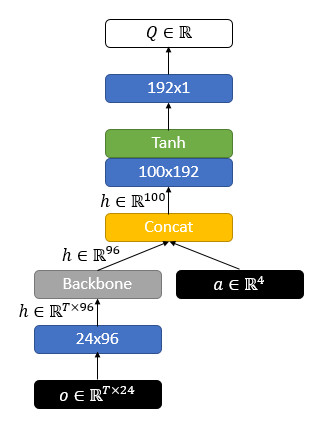
\includegraphics[width=0.65\linewidth]{figures/nets/critic.png}
		\caption{Critic Architecture}
		\label{fig:critic_net}
	\end{subfigure}
	\begin{subfigure}{.45\textwidth}
		\centering
		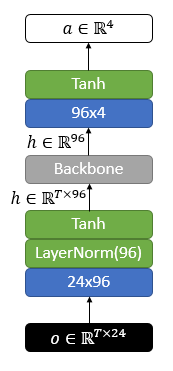
\includegraphics[width=0.4\linewidth]{figures/nets/actor.png}
		\caption{Actor Architecture}
		\label{fig:actor_net}
	\end{subfigure}
	\caption{Neural Architecture Design}
	\label{fig:nets}
\end{figure}
\end{frame}

\subsection{Residual Feed Forward Neural Network}

\begin{frame}
\frametitle{Residual Feed Forward Neural Network}
\begin{columns}[onlytextwidth]
	\begin{column}{.49\textwidth}
		\begin{itemize}
			\item As Feed Forward Networks becomes deeper, optimizing weights gets difficult. 
			\item For a 2 stacked layer (single skip connection), input and output of the stack is summed up for next calculations. 
			\item We have 2 layers with 192 dimensional hidden size and 96 dimensional output (single skip connection), 
			\item GELU as activation function.
			\item In our work, only last observation is feeded. 
		\end{itemize}
	\end{column}
	\begin{column}{.49\textwidth}
		\begin{figure}
			\centering
			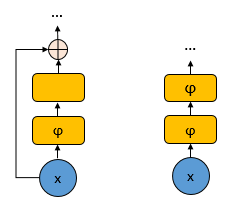
\includegraphics[width=0.6\textwidth]{figures/ml_theory/rffnn_vs_ffnn.png}
			\caption{Deep Feed Forward (left) and Deep Residual Feed Forward Network with single skip connection (right)}
			\label{fig:rffnn_ffnn}
		\end{figure}
	\end{column}
\end{columns}
\end{frame}

%%%%%%%%%%%%%%%%%%%%

\subsection{Long Short Term Memory}
\begin{frame}
\frametitle{Long Short Term Memory}
\begin{columns}[onlytextwidth]
	\begin{column}{.49\textwidth}
		\begin{itemize}
			\item Recurrent type of neural network.
			\item Explicitly designed to allow learning long-term dependencies.
			\item In our work, last 6 and 12 (only for SAC) observations are feeded. 
		\end{itemize}
	\end{column}
	\begin{column}{.49\textwidth}
		\begin{figure}
			\centering
			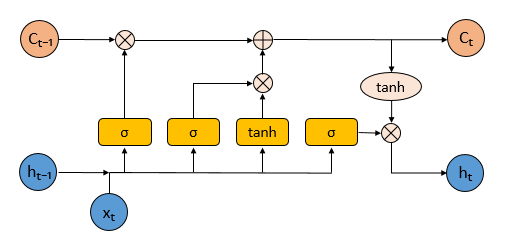
\includegraphics[width=0.95\textwidth]{figures/ml_theory/lstm_cell.png}
			\caption{LSTM Cell}
			\label{fig:lstm_cell}
		\end{figure}
	\end{column}
\end{columns}
\end{frame}

%%%%%%%%%%%%%%%%%%%%

\subsection{Transformer (Pre-layer Normalized)}
\begin{frame}
\frametitle{Transformer}
\begin{columns}[onlytextwidth]
	\begin{column}{.49\textwidth}
		\begin{itemize}
			\item Attention based neural network.
			\item Processes whole sequence at the same time.
			\item Uses positional encodings to encode order information.
			\item In our work, last 6 and 12 (only for SAC) observations are feeded. 			
		\end{itemize}
	\end{column}
	\begin{column}{.49\textwidth}
		\begin{figure}
			\centering
			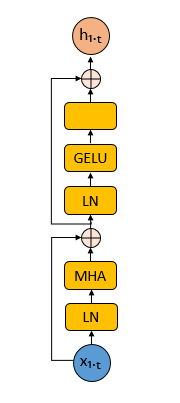
\includegraphics[width=0.4\textwidth]{figures/ml_theory/transformer_block.png}
			\caption{Pre-LN Transformer encoder layer with GELU activation}
			\label{fig:pre_trsf}
		\end{figure}
	\end{column}
\end{columns}
\end{frame}

%%%%%%%%%%%%%%%%%%%%
%%%%%%%%%%%%%%%%%%%%

\section{Algorithm Settings}
\begin{frame}
\frametitle{Algorithm Settings}
\begin{itemize}
	\item Hyperparameters are selected after a trial-error process considering literature. 
	\item Adam optimizer is used for optimization. 
	\item In TD3, as exploration noise, Ornstein-Uhlenbeck noise is used, and standart deviation is multiplied  by $0.9995$ at the end of each episode. 
	\item In SAC model, squashed gaussian policy is implemented. Therefore, along with layer giving mean actions, an additive layer is implemented for standart deviation along with it. 
	\item 8000 episodes for each training session. 
	\item Training sessions are run by multiple times to make comparison fair among models since some training sessions failed to converge and some yield worse results.
\end{itemize}
\end{frame}

%%%%%%%%%%%%%%%%%%%%
%%%%%%%%%%%%%%%%%%%%

\section{Results}

\begin{frame}
\frametitle{TD3 Results}
\begin{columns}[onlytextwidth]
	\begin{column}{.49\textwidth}
		\begin{figure}[!ht]
			\centering
			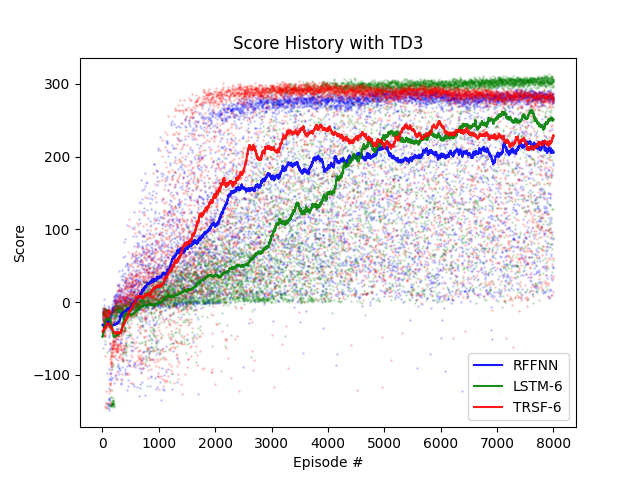
\includegraphics[width=0.99\textwidth]{figures/bipedal/SCT_TD3_RFFNN_LSTM-6_TRSF-6.png}
			\caption{Scatter Plot with Moving Average for Episode Scores (Window length: 200 episodes) for TD3}
			\label{fig:td3_scatter_ep_rewards}
		\end{figure}
	\end{column}
	\begin{column}{.49\textwidth}
		\begin{figure}[!ht]
			\centering
			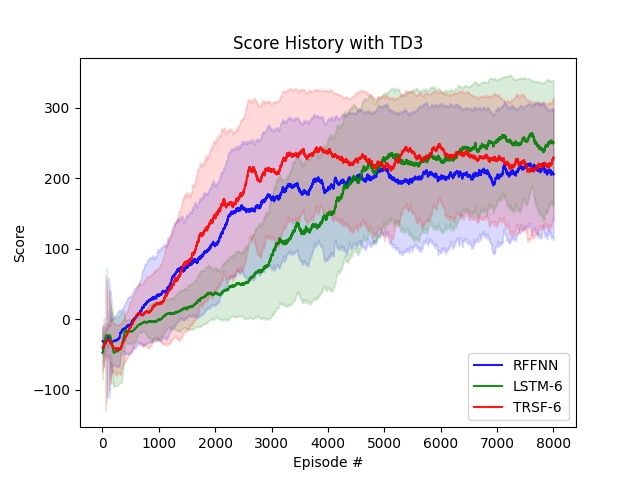
\includegraphics[width=0.99\textwidth]{figures/bipedal/STD_TD3_RFFNN_LSTM-6_TRSF-6.png}
			\caption{Moving Average and Standard Deviation for Episode Scores (Window length: 200 episodes) for TD3}
			\label{fig:td3_std_ep_rewards}
		\end{figure} 
	\end{column}
\end{columns}
\end{frame}

\begin{frame}
\frametitle{SAC Results}
\begin{columns}[onlytextwidth]
	\begin{column}{.49\textwidth}
		\begin{figure}[!ht]
			\centering
			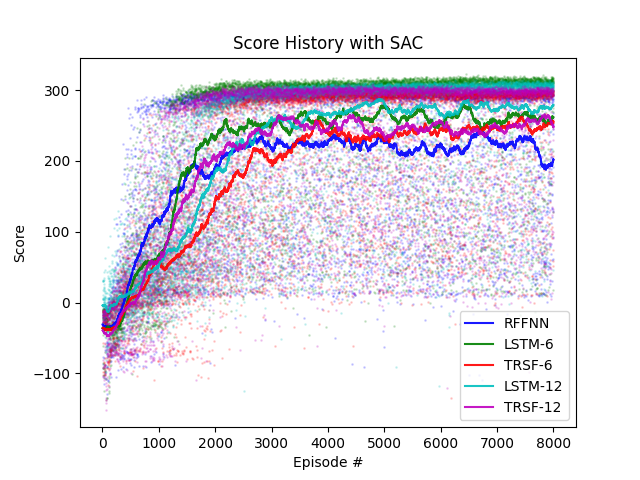
\includegraphics[width=0.95\textwidth]{figures/bipedal/SCT_SAC_RFFNN_LSTM-6_TRSF-6_LSTM-12_TRSF-12.png}
			\caption{Scatter Plot with Moving Average for Episode Scores (Window length: 200 episodes) for SAC}
			\label{fig:sac_scatter_ep_rewards}
		\end{figure}
	\end{column}
	\begin{column}{.49\textwidth}
		\begin{figure}[!ht]
			\centering
			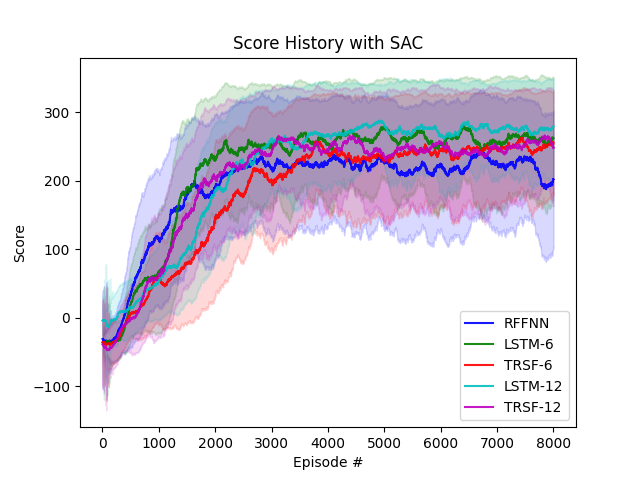
\includegraphics[width=0.95\textwidth]{figures/bipedal/STD_SAC_RFFNN_LSTM-6_TRSF-6_LSTM-12_TRSF-12.png}
			\caption{Moving Average and Standard Deviation for Episode Scores (Window length: 200 episodes) for SAC}
			\label{fig:sac_std_ep_rewards}
		\end{figure} 
	\end{column}
\end{columns}
\end{frame}

\begin{frame}
\frametitle{Test Performances of Best Checkpoints}
\begin{table}
	\begin{center}
		\caption{Best checkpoint performances with 100 test simulations}
		\begin{tabular}{||c c c c||} 
			\hline
			RL Method & Model & Episode & Avg. Score \\ [0.5ex] 
			\hline\hline
			TD3 & RFFNN & 6600 & 207 \\ 
			\hline
			SAC & RFFNN & 7600 & 219 \\
			\hline
			TD3 & TRSF-6 & 6400 & 222 \\
			\hline
			SAC & TRSF-6 & 6800 & 254 \\
			\hline
			SAC & TRSF-12 & 6000 & 270 \\
			\hline
			TD3 & LSTM-6 & 7000 & 242 \\
			\hline
			SAC & LSTM-6 & 7600 & 268 \\
			\hline
			SAC & LSTM-12 & 7200 & 298 \\ [1ex] 
			\hline
		\end{tabular}
		\label{table:ckpt_performance}
	\end{center}
\end{table}
\end{frame}

\begin{frame}
\frametitle{RFFNN Agent with SAC}
\begin{figure}[!ht]
	\centering
	\begin{subfigure}{.95\textwidth}
		\centering
		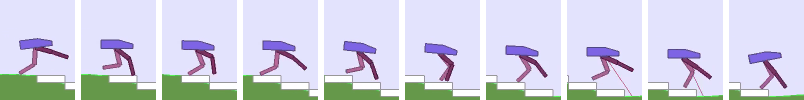
\includegraphics[width=0.95\textwidth]{figures/bipedal/anim/ff-stairs.png}
		\label{fig:anim_rffnn_stairs}
	\end{subfigure}
	\begin{subfigure}{.95\textwidth}
		\centering
		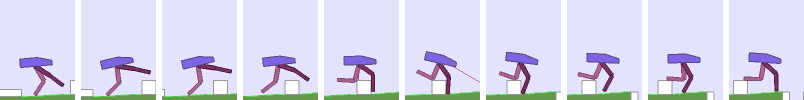
\includegraphics[width=0.95\textwidth]{figures/bipedal/anim/ff-hurdle.png}
		\label{fig:anim_rffnn_hurdle}
	\end{subfigure}
	\begin{subfigure}{.95\textwidth}
		\centering
		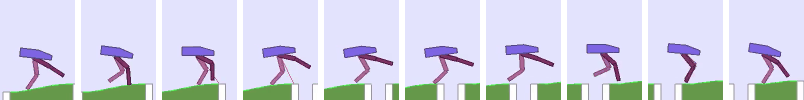
\includegraphics[width=0.95\textwidth]{figures/bipedal/anim/ff-pitfall.png}
		\label{fig:anim_rffnn_pitfall}
	\end{subfigure}
	\caption{Walking Simulation of RFFNN model at best version with SAC}
	\label{fig:rffnn_simulation}
\end{figure}
\end{frame}

\begin{frame}
\frametitle{LSTM-12 Agent with SAC}
\begin{figure}[!ht]
	\centering
	\begin{subfigure}{.95\textwidth}
		\centering
		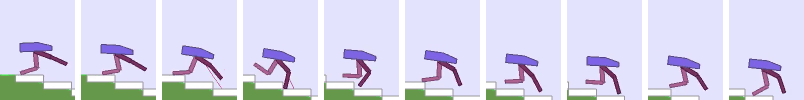
\includegraphics[width=0.95\textwidth]{figures/bipedal/anim/lstm-12-stairs.png}
		\label{fig:anim_lstm_stairs}
	\end{subfigure}
	\begin{subfigure}{.95\textwidth}
		\centering
		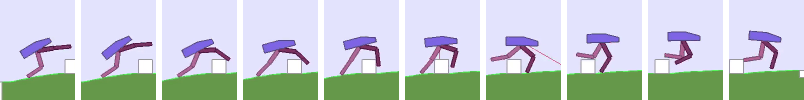
\includegraphics[width=0.95\textwidth]{figures/bipedal/anim/lstm-12-hurdle.png}
		\label{fig:anim_lstm_hurdle}
	\end{subfigure}
	\begin{subfigure}{.95\textwidth}
		\centering
		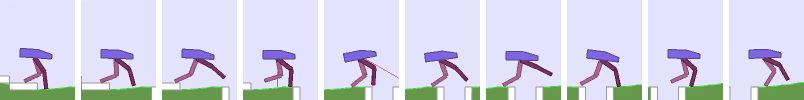
\includegraphics[width=0.95\textwidth]{figures/bipedal/anim/lstm-12-pitfall.png}
		\label{fig:anim_lstm_pitfall}
	\end{subfigure}
	\caption{Walking Simulation of LSTM-12 model at best version with SAC}
	\label{fig:lstm_simulation}
\end{figure}
\end{frame}

\begin{frame}
\frametitle{Transformer-12 Agent with SAC}
\begin{figure}[!ht]
	\centering
	\begin{subfigure}{.95\textwidth}
		\centering
		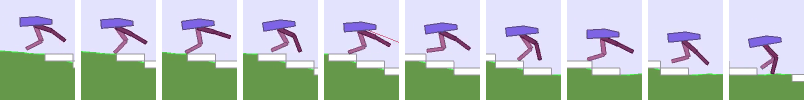
\includegraphics[width=0.95\textwidth]{figures/bipedal/anim/trsf-12-stairs.png}
		\label{fig:anim_trsf_stairs}
	\end{subfigure}
	\begin{subfigure}{.95\textwidth}
		\centering
		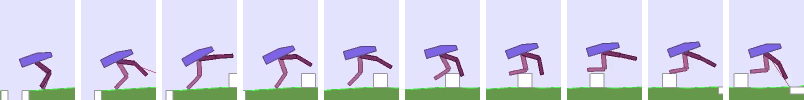
\includegraphics[width=0.95\textwidth]{figures/bipedal/anim/trsf-12-hurdle.png}
		\label{fig:anim_trsf_hurdle}
	\end{subfigure}
	\begin{subfigure}{.95\textwidth}
		\centering
		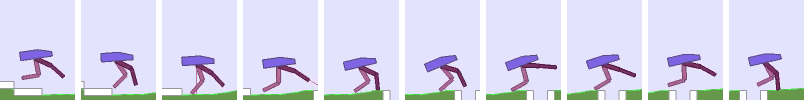
\includegraphics[width=0.95\textwidth]{figures/bipedal/anim/trsf-12-pitfall.png}
		\label{fig:anim_trsf_pitfall}
	\end{subfigure}
	\caption{Walking Simulation of Transformer-12 model at best version with SAC}
	\label{fig:trsf_simulation}
\end{figure}
\end{frame}

\begin{frame}
\frametitle{RFFNN Agent with SAC}
\begin{center}
\movie[height = 0.6\textwidth, width = 0.8\textwidth, poster, showcontrols] {}{video/ff-sac.mp4}
\end{center} 
\end{frame}

\begin{frame}
\frametitle{LSTM-12 Agent with SAC}
\begin{center}
\movie[height = 0.6\textwidth, width = 0.8\textwidth, poster, showcontrols] {}{video/lstm-12-sac.mp4}
\end{center} 
\end{frame}

\begin{frame}
\frametitle{Transformer-12 Agent with SAC}
\begin{center}
\movie[height = 0.6\textwidth, width = 0.8\textwidth, poster, showcontrols] {}{video/trsf-12-sac.mp4}
\end{center} 
\end{frame}

\section{Conclusion}
\begin{frame}
\frametitle{Conclusion}
\begin{itemize}
	\item LSTM is better than Transformers at least for our environment.
	\item Transformer can be used for RL problems.
	\item Using observation history improved performance.
	\item Environment modifications (rewarding, done signal etc.) are also source of such performance. 
	\item SAC is superior to TD3 for our environment thanks to better exploration logic.
\end{itemize}
\end{frame}

\begin{frame}{}
\centering \Huge
\emph{Thank You}
\end{frame}

% All of the following is optional and typically not needed.
\appendix
%%%%%%%%%%%%%%%%%%%%
%%%%%%%%%%%%%%%%%%%%
\section<presentation>*{\appendixname}
\subsection<presentation>*{For Further Reading}
\begin{frame}

\end{frame}
%%%%%%%%%%%%%%%%%%%%
%%%%%%%%%%%%%%%%%%%%
\section[References]{References}
\begin{frame}[t,allowframebreaks]
 %\frametitle<presentation>{For Further Reading}
%\tiny
%\centerslidesfalse
%\frametitle{REFERENCES}
%\bibliographystyle{amsalpha}
\bibliographystyle{apalike}
%\bibliographystyle{abbrvnat}
\bibliography{myBiblio}
\end{frame}

\end{document}


